\documentclass[11pt]{article}

% ── Packages ──────────────────────────────────────────────────────────────────
\usepackage[T1]{fontenc}
\usepackage[margin=1in]{geometry}
\usepackage{amsmath, amssymb, amsthm}
\usepackage{booktabs}
\usepackage{graphicx}
\graphicspath{{../results/plots/}}
\usepackage{hyperref}
\usepackage{microtype}
\usepackage{xcolor}
\usepackage[numbers,sort&compress]{natbib}
\usepackage{caption}
\usepackage{subcaption}
\usepackage{multirow}
\usepackage{array}
\usepackage{algorithm}
\usepackage{algorithmic}

% ── Theorem environments ───────────────────────────────────────────────────────
\newtheorem{theorem}{Theorem}[section]
\newtheorem{proposition}[theorem]{Proposition}
\newtheorem{corollary}[theorem]{Corollary}
\newtheorem{lemma}[theorem]{Lemma}
\newtheorem{definition}[theorem]{Definition}
\newtheorem{remark}[theorem]{Remark}

% ── Notation macros ────────────────────────────────────────────────────────────
\newcommand{\bx}{\mathbf{x}}
\newcommand{\by}{\mathbf{y}}
\newcommand{\bW}{\mathbf{W}}
\newcommand{\bh}{\mathbf{h}}
\newcommand{\orbsp}{\mathrm{orb}_{\mathrm{sp}}}
\newcommand{\orbco}{\mathrm{orb}_{\mathrm{co}}}
\newcommand{\Ocal}{\mathcal{O}}
\newcommand{\Gcal}{\mathcal{G}}
\newcommand{\R}{\mathbb{R}}
\newcommand{\abs}[1]{\left|#1\right|}

% ── Hyperref setup ─────────────────────────────────────────────────────────────
\hypersetup{
  colorlinks=true,
  linkcolor=blue!60!black,
  citecolor=green!50!black,
  urlcolor=blue!60!black
}

% ─────────────────────────────────────────────────────────────────────────────
\title{\textbf{Exploiting Spatial and Color Symmetry in Equivariant\\
Value Networks for the 2\texttimes2\texttimes2 Pocket Cube}}

\author{Zhambyl Maksotov, Miras Abdykhali, Adilbek Moldabek\\
\small Research Methods\\
\small Nazarbayev University}

\date{\today}
% ─────────────────────────────────────────────────────────────────────────────

\begin{document}
\maketitle

% ── MSC / Keywords ────────────────────────────────────────────────────────────
\noindent\textbf{MSC 2020:} 68T07 (Artificial intelligence, machine learning);
20B30 (Symmetric groups);
68R10 (Graph theory in computer science)

\medskip
\noindent\textbf{Keywords:} equivariant neural networks, group symmetry,
combinatorial puzzle, value function, beam search

\medskip
\noindent\textbf{AI use statement:}
The authors used Claude (Anthropic) to assist with \LaTeX{} formatting,
proof editing, and code generation for the experimental pipeline.
All theoretical content, experimental design, and interpretation of results
are the authors' own work.

% ── Abstract ──────────────────────────────────────────────────────────────────
\begin{abstract}
Learning value functions for combinatorial search problems requires models
that generalize reliably across symmetry-equivalent states.
The 2\texttimes2\texttimes2 Pocket Cube possesses two physically meaningful
symmetry groups: the 24-element rotation group $\mathcal{O}$ (spatial
orientations) and the 720-element symmetric group $S_6$ (color relabelings),
whose direct product $\mathcal{G} = \mathcal{O} \times S_6$ has
$17{,}280$ elements.
We design and analyze two group-equivariant architectures:
\textsc{EMLP} (equivariant to $\mathcal{O}$, ${\sim}$42K parameters) and
\textsc{EMLP-Col} (equivariant to the full $\mathcal{G}$, ${\sim}$39K parameters),
compared against a large unconstrained \textsc{MLP} (${\sim}$169K
parameters) as the no-symmetry baseline.
We prove that both architectures are exactly invariant to their respective
symmetry groups and show that equivariance to $\mathcal{G}$ implicitly
provides $17{,}280$-fold data augmentation.
Empirically, \textsc{EMLP-Col} achieves a greedy
solve rate of 97.2\% at scramble depth 10 and a mean absolute error of
0.932 moves, compared to 94.2\% and 1.239 moves for the spatial-only
\textsc{EMLP}, and a solve rate of 0.0\% for the unconstrained \textsc{MLP}.
The results show that building in symmetry directly—rather than leaving it
for the model to learn from data—produces more consistent value landscapes
that are critical for reliable beam-search guided solving.
\end{abstract}

% ── 1. Introduction ───────────────────────────────────────────────────────────
\section{Introduction}
\label{sec:intro}

Combinatorial puzzles offer a clean testbed for evaluating how well neural
networks exploit problem structure.
Unlike most learning tasks where symmetry is approximate or data-driven,
combinatorial puzzles often have exact, group-theoretic symmetry baked
into their definition—symmetry that, if ignored, forces a model to rediscover
the same relationships from data across every equivalent configuration.

The 2\texttimes2\texttimes2 Pocket Cube is an
especially attractive benchmark: its state space of 3,674,160 reachable
configurations is small enough to solve exactly via breadth-first search
(BFS), yielding ground-truth distances for every state
\cite{agostinelli2019solving}.
A value network $f: \R^{144} \to \R$ that predicts BFS distance can guide
greedy or beam search to solve scrambled cubes without tree search or
explicit rollouts.

\paragraph{Two symmetries of the cube.}
The cube has two physically meaningful symmetry groups:
\begin{itemize}
  \item \textbf{Spatial rotations $\mathcal{O}$} (order 24): rotating the
    entire physical cube does not change its distance to the solved state.
    Any value function must satisfy $f(\pi \cdot \bx) = f(\bx)$ for all
    $\pi \in \mathcal{O}$.
  \item \textbf{Color permutations $S_6$} (order 720): systematically
    relabeling all six colors yields an isomorphic puzzle with identical
    structure.
    Thus $f(\sigma \cdot \bx) = f(\bx)$ for all $\sigma \in S_6$.
\end{itemize}
Together these form the group $\mathcal{G} = \mathcal{O} \times S_6$ of
order $24 \times 720 = 17{,}280$.
An unconstrained MLP must learn all $17{,}280$ equivalent views from data;
an equivariant model encodes them exactly by construction.

\paragraph{Beam search as the evaluation criterion.}
A value network is only useful insofar as it guides a solver to the solved
state.
Recent work by Chervov et al.~\cite{chervov2025cayleypy} (the CayleyPy project)
demonstrates that beam search guided by a learned distance heuristic
is the most effective strategy for solving Rubik's cubes of all sizes,
achieving 98.4\% optimality on the standard $3{\times}3{\times}3$ cube and
surpassing all prior methods—including DeepCubeA \cite{agostinelli2019solving}
(60.3\% optimality) and EfficientCube \cite{efficientcube} (69.6\%
optimality)—while being $26\times$ faster.
Crucially, Chervov et al.\ characterize the symbiotic role of the two
components: \emph{``The neural network provides heuristics on where to make
the next steps, while the graph pathfinding technique compensates for any
possible incorrectness in the neural network predictions.''}
This framing directly motivates our evaluation strategy: we measure value
network quality through beam search solve rate, because a good heuristic
should produce a reliable value landscape for local move selection, even
under a modest beam width.

\paragraph{Contributions.}
We make the following contributions:
\begin{enumerate}
  \item We design a \textbf{Color-Equivariant Convolution layer}
    (\textsc{ColorConv}) that is jointly equivariant to
    $\mathcal{G} = \mathcal{O} \times S_6$, using a block-of-six channel
    structure to represent $S_6$ acting on the color dimension.
  \item We provide \textbf{formal proofs} of equivariance for both the
    spatial-only layer (\textsc{SpatialConv}) and the combined layer
    (\textsc{ColorConv}), and a corollary establishing invariance of
    the complete networks.
  \item We show that equivariance to $\mathcal{G}$ is equivalent to
    \textbf{implicit $17{,}280$-fold data augmentation}—a strictly stronger
    guarantee than explicit augmentation.
  \item We demonstrate empirically that at equal parameter count (${\sim}$40K),
    the equivariant models substantially outperform an unconstrained
    \textsc{MLP} on every metric, and expose the \textbf{``local consistency
    gap''}: symmetry matters not just for average prediction accuracy but for
    the per-move ranking consistency that beam search depends on.
\end{enumerate}

\paragraph{Paper structure.}
Section~\ref{sec:background} introduces the 2\texttimes2\texttimes2 cube,
the relevant group theory, and the general framework of equivariant networks.
Section~\ref{sec:related} surveys related work on neural cube solvers,
beam-search heuristics, and equivariant architectures.
Section~\ref{sec:method} describes the two equivariant layers
(\textsc{SpatialConv} and \textsc{ColorConv}), the invariant pooling heads,
the full model architectures, and training setup.
Section~\ref{sec:theory} provides formal proofs of equivariance and
invariance, and establishes the implicit data-augmentation guarantee.
Section~\ref{sec:experiments} presents the experimental design, evaluation
metrics, and results.
Section~\ref{sec:discussion} discusses the findings and limitations.
Section~\ref{sec:conclusion} concludes.

% ── 2. Background ─────────────────────────────────────────────────────────────
\section{Background}
\label{sec:background}

\subsection{The 2\texttimes2\texttimes2 Pocket Cube}

\begin{figure}[t]
  \centering
  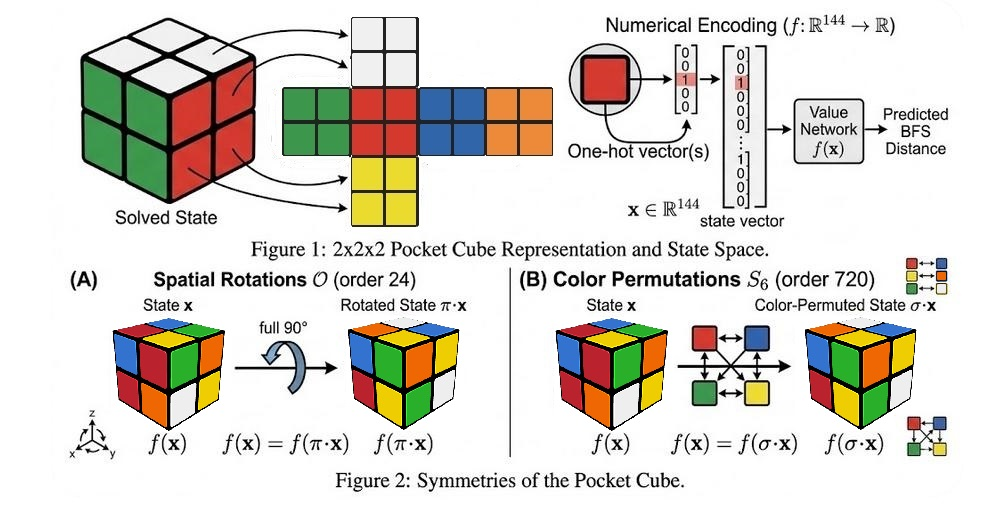
\includegraphics[width=\linewidth]{RM-2x2.jpg}
  \caption{Top: the 2\texttimes2\texttimes2 Pocket Cube, its unfolded sticker
    representation, one-hot encoding $\bx \in \R^{144}$, and the value network
    $f(\bx)$ predicting BFS distance.
    Bottom: the two symmetry groups exploited in this work —
    spatial rotations $\mathcal{O}$ (order 24) and color permutations $S_6$
    (order 720) — both of which leave BFS distance invariant.}
  \label{fig:cube}
\end{figure}

The 2\texttimes2\texttimes2 cube has 6 faces, each divided into 4 stickers,
giving 24 sticker positions (Figure~\ref{fig:cube}).
We index positions $i \in \{1, \ldots, 24\}$ and colors
$c \in \{1, \ldots, 6\}$.
A state $\bx \in \{0,1\}^{24 \times 6}$ is a one-hot matrix where
$x_{i,c} = 1$ if sticker $i$ shows color $c$.
We flatten $\bx$ to a vector of dimension $144$ as network input.

The move set consists of six quarter-turn moves
$\{R, R', U, U', F, F'\}$ in the quarter-turn metric (QTM).
BFS over the Cayley graph of all 3,674,160 reachable states establishes
God's number: the maximum BFS distance is $d_{\max} = 14$ in QTM
\cite{jaapsch2x2, rokicki2014diameter}.
The exact distance $d(\bx) \in \{0, 1, \ldots, 14\}$ for every state can
be precomputed and stored in a lookup table, providing noiseless supervision
for training a value network $f(\bx) \approx d(\bx)$.

\subsection{Group Theory}

\begin{definition}[Group action]
A group $G$ \emph{acts} on a set $X$ if there is a map
$G \times X \to X$, $(g, x) \mapsto g \cdot x$, satisfying
$e \cdot x = x$ and $(gh) \cdot x = g \cdot (h \cdot x)$ for all
$g, h \in G$ and $x \in X$.
\end{definition}

\begin{definition}[Orbit]
The \emph{orbit} of $x \in X$ under $G$ is
$G \cdot x = \{g \cdot x : g \in G\}$.
Two elements $x, x' \in X$ lie in the same orbit iff $\exists g \in G$
such that $g \cdot x = x'$.
\end{definition}

\paragraph{The rotation group $\mathcal{O}$.}
The rotation group of the cube, $\mathcal{O}$, has 24 elements.
Each $\pi \in \mathcal{O}$ acts on sticker positions as a permutation
$\pi: \{1,\ldots,24\} \to \{1,\ldots,24\}$.
The induced action on states is
\begin{equation}
  [\pi \cdot \bx]_{i,c} = x_{\pi^{-1}(i),\, c}.
  \label{eq:spatial_action}
\end{equation}
We represent $\mathcal{O}$ by its Cayley generators: a $90^\circ$ rotation
around the right-left axis ($R_{90}$) and around the up-down axis ($U_{90}$).

\paragraph{The color permutation group $S_6$.}
The symmetric group $S_6$ consists of all $6! = 720$ permutations of the six
colors.
Each $\sigma \in S_6$ acts on states by permuting the color channels:
\begin{equation}
  [\sigma \cdot \bx]_{i,c} = x_{i,\, \sigma^{-1}(c)}.
  \label{eq:color_action}
\end{equation}

\paragraph{The combined group $\mathcal{G} = \mathcal{O} \times S_6$.}
The \emph{direct product} of $\mathcal{O}$ and $S_6$ has order
$24 \times 720 = 17{,}280$.
An element $(g, \sigma) \in \mathcal{G}$ acts on states as
\begin{equation}
  [(g, \sigma) \cdot \bx]_{i,c} = x_{g^{-1}(i),\; \sigma^{-1}(c)}.
  \label{eq:combined_action}
\end{equation}
Because the cube's distance to the solved state is unchanged by rotating
the physical cube or relabeling all colors, $d(\bx) = d((g, \sigma) \cdot \bx)$
for all $(g, \sigma) \in \mathcal{G}$.

\begin{definition}[Equivariant and invariant maps]
A map $f: X \to Y$ is \emph{$G$-equivariant} if
$f(g \cdot x) = g \cdot f(x)$ for all $g \in G$, $x \in X$,
where $G$ acts on both $X$ and $Y$.
If $G$ acts trivially on $Y$ (i.e., $g \cdot y = y$), then
$f(g \cdot x) = f(x)$ and $f$ is called \emph{$G$-invariant}.
\end{definition}

The value network $f: \R^{144} \to \R$ should be $\mathcal{G}$-invariant.

\subsection{Equivariant Neural Networks}

Equivariant networks build invariance or equivariance directly into the
architecture by constraining layer weights via symmetry.
The key idea, originating with group-equivariant CNNs
\cite{cohen2016group}, is to use weight sharing across orbits:
parameters shared across all group-equivalent input-output pairs.
This simultaneously reduces the effective parameter count and guarantees
exact symmetry.

\paragraph{Pair orbits.}
For a group $G$ acting on an index set $\{1, \ldots, n\}$, the
\emph{pair orbits} are the equivalence classes of pairs $(i, j)$ under
\begin{equation}
  (i, j) \sim (i', j') \iff \exists g \in G : g(i) = i',\ g(j) = j'.
\end{equation}
The number of pair orbits determines the number of independent weight
parameters in a $G$-equivariant linear layer.
For $\mathcal{O}$ acting on 24 sticker positions, there are
$n_{\mathrm{sp}} = 24$ spatial pair orbits.
For $S_6$ acting on 6 colors, there are only $n_{\mathrm{co}} = 2$
color pair orbits: the orbit of diagonal pairs $(c, c)$ and the orbit of
off-diagonal pairs $(c, c')$ with $c \neq c'$.

% ── 3. Related Work ───────────────────────────────────────────────────────────
\section{Related Work}
\label{sec:related}

\paragraph{Neural solvers for Rubik's cubes.}
Agostinelli et al.~\cite{agostinelli2019solving} introduced DeepCubeA, which
trains a value network via autodidactic iteration (a form of self-supervised
reinforcement learning) and uses it to guide A* search.
Although DeepCubeA solves the $3{\times}3{\times}3$ cube, it achieves only
60.3\% solution optimality and requires substantial computation.
McAleer et al.~\cite{mcaleer2019solving} improved upon this with approximate
policy iteration.
These works establish that a learned heuristic can successfully guide search
for combinatorial puzzles, but they do not exploit the cube's symmetry
structure in the architecture.

\paragraph{Beam search with learned heuristics.}
The CayleyPy project \cite{chervov2025cayleypy} is the most directly relevant
recent work to our evaluation methodology.
Chervov et al.\ propose a general framework in which a neural network estimates
a ``diffusion distance'' to the solved state, and beam search of width
$W$ uses these estimates to maintain the $W$ most promising frontier states at
each step.
They demonstrate that this combination achieves 98.4\% optimality on the
$3{\times}3{\times}3$ cube (versus 60.3\% for DeepCubeA) and scales to cubes
up to $5{\times}5{\times}5$—well beyond the reach of any prior method.
A key finding is that solution quality improves approximately linearly with
$\log W$, suggesting that heuristic accuracy governs the fundamental
efficiency of the approach: a more accurate value function allows a narrower
beam to succeed.
Chervov et al.\ explicitly note that \emph{``the neural network provides
heuristics on where to make the next steps, while the graph pathfinding
technique compensates for any possible incorrectness in the neural network
predictions''}, highlighting that beam search is robust to moderate heuristic
error but ultimately bottlenecked by heuristic consistency at the local level.
This motivates our use of beam search solve rate—rather than MAE or Pearson
$r$ alone—as the primary metric for comparing value network quality: a
consistent, equivariant value landscape should translate directly into higher
solve rates even under a narrow beam.

\paragraph{Equivariant networks for combinatorial structures.}
Cohen and Welling~\cite{cohen2016group} established the general framework of
group-equivariant CNNs.
Finzi et al.~\cite{finzi2021practical} provide a practical implementation
for arbitrary matrix groups via the EMLP framework.
Kondor and Trivedi~\cite{kondor2018generalization} show that equivariance
to compact groups can be enforced through convolution on the group.
Maron et al.~\cite{maron2020learning} study equivariant networks for sets
and symmetric structures more generally.
Our work applies these ideas to the specific symmetry group of the Pocket
Cube and introduces a novel weight-sharing scheme for the product group
$\mathcal{O} \times S_6$.

% ── 4. Method ─────────────────────────────────────────────────────────────────
\section{Method}
\label{sec:method}

\subsection{Spatial Group Convolution Layer (\textsc{SpatialConv})}
\label{sec:groupconv}

The \textsc{SpatialConv} layer maps a hidden state of shape
$(B, 24, c_{\mathrm{in}})$ to $(B, 24, c_{\mathrm{out}})$, where $B$
is the batch dimension and the 24-position axis carries the sticker
representation.

\paragraph{Weight sharing.}
Let $\orbsp: \{1,\ldots,24\}^2 \to \{1,\ldots,n_{\mathrm{sp}}\}$ map each
position pair $(i,j)$ to its orbit index under $\mathcal{O}$.
The layer has a weight tensor
$\bW \in \R^{c_{\mathrm{out}} \times c_{\mathrm{in}} \times n_{\mathrm{sp}}}$
and a bias $\boldsymbol{\beta} \in \R^{c_{\mathrm{out}}}$.
The full $24 \times 24$ kernel is obtained by index-gathering:
\begin{equation}
  K_{o, c, i, j} = W_{o,\, c,\, \orbsp(i, j)},
  \qquad
  o \in [c_{\mathrm{out}}],\ c \in [c_{\mathrm{in}}],\ i, j \in [24].
\end{equation}

\paragraph{Forward pass.}
\begin{equation}
  y_{b,i,o} = \sum_{j=1}^{24} \sum_{c=1}^{c_{\mathrm{in}}}
              K_{o,c,i,j} \cdot x_{b,j,c} + \beta_o.
  \label{eq:groupconv_forward}
\end{equation}

\paragraph{Parameter count.}
$c_{\mathrm{out}} \times c_{\mathrm{in}} \times 24 + c_{\mathrm{out}}$,
compared to $c_{\mathrm{out}} \times c_{\mathrm{in}} \times 24^2$ for an
unconstrained layer of the same width — a $24\times$ reduction.

\subsection{Color-Equivariant Convolution Layer (\textsc{ColorConv})}
\label{sec:colorconv}

The \textsc{ColorConv} layer is the main technical contribution of this
paper.
It extends \textsc{SpatialConv} to the full group
$\mathcal{G} = \mathcal{O} \times S_6$.

\paragraph{Block-of-six channel structure.}
To enable $S_6$ to act naturally on the hidden representation, we organize
channels in blocks of six: a hidden state with $k$ blocks has
$6k$ total channels, grouped as a tensor of shape
$(B, 24, k, 6)$, where the last axis carries a 6-dimensional representation
of $S_6$.
Under $(g, \sigma) \in \mathcal{G}$, the hidden state transforms as
\begin{equation}
  [(g, \sigma) \cdot \bh]_{b,i,\kappa,d} = h_{b,\, g^{-1}(i),\, \kappa,\, \sigma^{-1}(d)}.
  \label{eq:hidden_action}
\end{equation}

\paragraph{Color pair orbits.}
Under the conjugation action of $S_6$ on pairs $(d, c) \in \{1,\ldots,6\}^2$,
there are exactly two orbits:
\begin{equation}
  \orbco(d, c) =
  \begin{cases}
    0 & \text{if } d = c \quad \text{(same color, 6 pairs)}, \\
    1 & \text{if } d \neq c \quad \text{(different colors, 30 pairs)}.
  \end{cases}
  \label{eq:color_orbits}
\end{equation}
This follows from the fact that $S_6$ acts transitively on all same-color
pairs and on all different-color pairs separately.

\paragraph{Weight tensor and kernel expansion.}
The layer has weight
$\bW \in \R^{k_{\mathrm{out}} \times k_{\mathrm{in}} \times n_{\mathrm{sp}} \times 2}$
and bias $\boldsymbol{\beta} \in \R^{k_{\mathrm{out}}}$.
The full $24 \times 24 \times 6 \times 6$ kernel is:
\begin{equation}
  K_{o,\kappa,i,j,d,c} = W_{o,\; \kappa,\; \orbsp(i,j),\; \orbco(d,c)}.
  \label{eq:colorconv_kernel}
\end{equation}

\paragraph{Forward pass.}
\begin{equation}
  y_{b,i,o,d} = \sum_{j=1}^{24} \sum_{\kappa=1}^{k_{\mathrm{in}}}
                \sum_{c=1}^{6} K_{o,\kappa,i,j,d,c} \cdot x_{b,j,\kappa,c}
                + \beta_o.
  \label{eq:colorconv_forward}
\end{equation}
The output is then reshaped to $(B, 24, 6\,k_{\mathrm{out}})$ for the next layer.

\paragraph{Parameter count.}
$k_{\mathrm{out}} \times k_{\mathrm{in}} \times n_{\mathrm{sp}} \times 2
+ k_{\mathrm{out}}$.
With $n_{\mathrm{sp}} = 24$ and channel width $6k$, this is
$24 \times 2 = 48$ independent weights per block pair — compared to
$(6k)^2 \times 24^2 = 20{,}736 k^2$ for an unconstrained layer,
a compression of \textbf{0.23\%} (for any $k$).

\subsection{Comparison with the General EMLP Framework}
\label{sec:emlp_comparison}

Both our layers and the general EMLP framework of Finzi et al.\
\cite{finzi2021practical} solve the same underlying mathematical problem:
characterising the space of $G$-equivariant linear maps
$\text{Hom}_G(V, W)$ between two group representations.
They differ in how that space is computed.

\paragraph{EMLP (Finzi et al.) — numerical approach.}
For a group $G$ with generators $\{g_i\}$, the equivariance constraint
$L\,\rho_\text{in}(g) = \rho_\text{out}(g)\,L$ on a linear map
$L \in \R^{|W| \times |V|}$ can be written as
\begin{equation}
  C\,\mathrm{vec}(L) = \mathbf{0},
  \qquad
  C = \bigoplus_i
  \Bigl(\rho_\text{in}(g_i)^\top \otimes I_{|W|}
        - I_{|V|} \otimes \rho_\text{out}(g_i)\Bigr).
  \label{eq:emlp_constraint}
\end{equation}
The equivariant basis $\{B_k\}$ is the \textbf{null space of} $C$,
found via Krylov iterations or SVD.
The layer is then parameterised as $L = \sum_k c_k B_k$ with learnable
scalars $\{c_k\}$.
This approach is fully general: it applies to any group (including
continuous groups such as SO(3) or SE(3)) and any representation, at the
cost of constructing and factorising $C$, which has size
$O(|V|^2 |W|^2)$.

\paragraph{Orbit enumeration (our approach) — combinatorial approach.}
For a finite group acting by permutation, the null space of
$C$ has a direct combinatorial description: by Schur's lemma, the entry
$L_{ij}$ depends only on the orbit of the pair $(i,j)$ under the group
action.
We therefore compute orbit indices directly by exhaustive enumeration
of the group,
\begin{equation}
  \mathrm{orb}(i,j) = \mathrm{orb}(i',j')
  \;\iff\;
  \exists\, g \in G : g(i)=i',\; g(j)=j',
  \label{eq:orbit_enum}
\end{equation}
and parameterise $L_{ij} = W_{\mathrm{orb}(i,j)}$ with one learnable
scalar per orbit.
The basis vectors are the orbit indicator matrices
$[B_k]_{ij} = \mathbf{1}[\mathrm{orb}(i,j)=k]$, which are exactly the
null-space basis that EMLP would recover numerically.

\paragraph{Equivalence and trade-offs.}
For finite permutation representations the two approaches produce
identical equivariant function classes: the null space of $C$
equals the span of the orbit indicator matrices.
For the 2\texttimes2\texttimes2 cube, $G = \mathcal{O}$ has only 24 elements
acting on 24 sticker positions.
Orbit enumeration computes all pair orbits in milliseconds with zero
floating-point error, making EMLP's Krylov machinery unnecessary.
The general EMLP framework becomes the right tool when the group is
continuous (e.g.\ learning a value function equivariant to SO(3) rotations
in 3D space) or when the representation is not a simple permutation action.

\subsection{Invariant Pooling Heads}

Both networks end with an invariant pooling head that reduces the
equivariant representation to a scalar.

\paragraph{Spatial pooling (for \textsc{EMLP}).}
Average over the 24 position axis, then apply a linear projection:
\begin{equation}
  f(\bx) = \mathbf{w}^\top \!\left(\frac{1}{24}\sum_{i=1}^{24} \bh_i\right) + b,
  \qquad \mathbf{w} \in \R^{c_{\mathrm{hidden}}}.
  \label{eq:invlinear}
\end{equation}

\paragraph{Spatial + color pooling (for \textsc{EMLP-Col}).}
Average over both the 24 positions and the 6 colors within each block,
then apply a linear projection:
\begin{equation}
  f(\bx) = \mathbf{w}^\top \!\left(\frac{1}{144}\sum_{i=1}^{24}\sum_{d=1}^{6}
            \bh_{i,\cdot,d}\right) + b,
  \qquad \mathbf{w} \in \R^{k_{\mathrm{hidden}}}.
  \label{eq:invhead}
\end{equation}

\subsection{Full Model Architectures}

Both equivariant models use 3 hidden layers with ReLU activations.
Table~\ref{tab:models} summarizes the three architectures compared in this work.

\begin{table}[h]
\centering
\caption{The three model architectures compared in this work.
All models use 3 hidden layers with ReLU activations.
Parameter counts use widths $c=28$ (\textsc{EMLP}), $k=20$ (\textsc{EMLP-Col}),
$h=110$ (\textsc{MLP}).
$^\dagger$Two additional baselines were evaluated but are not the primary focus:
an augmented \textsc{MLP} (\textsc{MLP-Aug}, $h=110$, ${\sim}$40K) and a large
unconstrained \textsc{MLP} ($h=256$, ${\sim}$169K); see footnote in
Table~\ref{tab:results}.}
\label{tab:models}
\renewcommand{\arraystretch}{1.2}
\begin{tabular}{lllrll}
\toprule
\textbf{Model} & \textbf{Layer type} & \textbf{Width} & \textbf{Params} &
  \textbf{Symmetry} & \textbf{Role} \\
\midrule
\textsc{EMLP}     & \textsc{SpatialConv}      & $c=28$ & $\sim$42K &
  $\mathcal{O}$             & Spatial equivariance \\
\textsc{EMLP-Col} & \textsc{ColorConv} & $k=20$ & $\sim$39K &
  $\mathcal{O} \times S_6$  & Spatial + color equivariance \\
\textsc{MLP}      & Linear                  & $h=110$& $\sim$40K &
  None                      & Parameter-matched baseline \\
\bottomrule
\end{tabular}
\end{table}

\paragraph{Input/output.}
All models accept a flattened one-hot state vector of dimension 144.
Equivariant models immediately reshape to $(24, 6)$ (or $(24, 1, 6)$ for
\textsc{EMLP-Col}) before processing.
All models output a scalar prediction $\hat{d} \in [0, 1]$, which is
scaled back to move units as $14 \cdot \hat{d}$.

\subsection{Training Setup}
\label{sec:training}

\paragraph{Dataset.}
We precompute exact BFS distances for all 3,674,160 reachable states.
The training set of 200,000 samples is drawn with equal probability from
each depth $d \in \{1, \ldots, 14\}$ (stratified).
The validation set has 20,000 randomly sampled states; the test set has
$\approx$1,000 states at each depth $d \in \{0, \ldots, 14\}$ ($\approx$15K
total).

\paragraph{Objective.}
We minimize mean squared error on normalized targets:
\begin{equation}
  \mathcal{L} = \frac{1}{N} \sum_{n=1}^{N}
    \left(f(\bx^{(n)}) - \frac{d(\bx^{(n)})}{14}\right)^2.
\end{equation}

\paragraph{Optimization.}
We use Adam \cite{kingma2015adam} with initial learning rate $10^{-3}$,
decayed via cosine annealing to $10^{-5}$ over 200 epochs.
Batch size is 512.
Early stopping is applied with patience 15 on validation MSE;
the best checkpoint is saved and used for evaluation.
All experiments use 3 independent random seeds (42, 43, 44) to estimate
variance.

% ── 4. Theoretical Analysis ───────────────────────────────────────────────────
\section{Theoretical Analysis}
\label{sec:theory}

\subsection{Equivariance of \textsc{SpatialConv}}

\begin{proposition}[\textsc{SpatialConv} is $\mathcal{O}$-equivariant]
\label{prop:groupconv}
Let $\pi \in \mathcal{O}$ act on sticker positions.
For any input $\bx \in \R^{B \times 24 \times c_{\mathrm{in}}}$,
\begin{equation}
  \textsc{SpatialConv}(\pi \cdot \bx) = \pi \cdot \textsc{SpatialConv}(\bx),
\end{equation}
where $[\pi \cdot \bx]_{b,i,c} = x_{b,\pi^{-1}(i),c}$ on the input
and $[\pi \cdot \by]_{b,i,o} = y_{b,\pi^{-1}(i),o}$ on the output.
\end{proposition}

\begin{proof}
Fix $b, i, o$.
By definition of pair orbits, for any $\pi \in \mathcal{O}$,
\begin{equation}
  \orbsp\!\left(\pi^{-1}(i),\, j'\right)
  = \orbsp\!\left(i,\, \pi(j')\right)
  \label{eq:orbit_invariance}
\end{equation}
for all $j' \in \{1,\ldots,24\}$.
(This holds because $(i, \pi(j'))$ and $(\pi^{-1}(i), j')$ are related by
the group element $\pi^{-1}$: $\pi^{-1}(i) = \pi^{-1}(i)$ and
$\pi^{-1}(\pi(j')) = j'$.)

We compute the $i$-th output of $\textsc{SpatialConv}(\pi \cdot \bx)$:
\begin{align}
  \left[\textsc{SpatialConv}(\pi \cdot \bx)\right]_{b,i,o}
  &= \sum_{j=1}^{24} \sum_{c=1}^{c_{\mathrm{in}}}
     W_{o,c,\,\orbsp(i,j)} \cdot [\pi \cdot \bx]_{b,j,c} \notag \\
  &= \sum_{j=1}^{24} \sum_{c=1}^{c_{\mathrm{in}}}
     W_{o,c,\,\orbsp(i,j)} \cdot x_{b,\pi^{-1}(j),c}.
\end{align}
Substituting $j' = \pi^{-1}(j)$ (so $j = \pi(j')$, and the sum still
ranges over all 24 positions):
\begin{align}
  &= \sum_{j'=1}^{24} \sum_{c=1}^{c_{\mathrm{in}}}
     W_{o,c,\,\orbsp(i,\,\pi(j'))} \cdot x_{b,j',c} \notag \\
  &\overset{\eqref{eq:orbit_invariance}}{=}
     \sum_{j'=1}^{24} \sum_{c=1}^{c_{\mathrm{in}}}
     W_{o,c,\,\orbsp(\pi^{-1}(i),\,j')} \cdot x_{b,j',c} \notag \\
  &= \left[\textsc{SpatialConv}(\bx)\right]_{b,\pi^{-1}(i),o}
   = \left[\pi \cdot \textsc{SpatialConv}(\bx)\right]_{b,i,o}. \qedhere
\end{align}
\end{proof}

\subsection{Equivariance of \textsc{ColorConv}}

\begin{theorem}[\textsc{ColorConv} is $\mathcal{G}$-equivariant]
\label{thm:colorconv}
Let $(g, \sigma) \in \mathcal{G} = \mathcal{O} \times S_6$ act as in
\eqref{eq:hidden_action}.
For any input $\bx \in \R^{B \times 24 \times k_{\mathrm{in}} \times 6}$,
\begin{equation}
  \textsc{ColorConv}\!\left((g,\sigma) \cdot \bx\right)
  = (g,\sigma) \cdot \textsc{ColorConv}(\bx).
\end{equation}
\end{theorem}

\begin{proof}
Fix $b, i, o, d$.
We compute the $(i, o, d)$-th output of
$\textsc{ColorConv}\!\left((g, \sigma) \cdot \bx\right)$:
\begin{align}
  \left[\textsc{ColorConv}\!\left((g,\sigma)\cdot\bx\right)\right]_{b,i,o,d}
  &= \sum_{j,\kappa,c} K_{o,\kappa,i,j,d,c}
     \cdot \left[(g,\sigma)\cdot\bx\right]_{b,j,\kappa,c} \notag \\
  &= \sum_{j,\kappa,c} W_{o,\kappa,\orbsp(i,j),\orbco(d,c)}
     \cdot x_{b,g^{-1}(j),\kappa,\sigma^{-1}(c)}.
\end{align}
Substituting $j' = g^{-1}(j)$ and $c' = \sigma^{-1}(c)$:
\begin{align}
  &= \sum_{j',\kappa,c'} W_{o,\kappa,\,\orbsp(i,\,g(j')),\,\orbco(d,\,\sigma(c'))}
     \cdot x_{b,j',\kappa,c'}.
  \label{eq:proof_step}
\end{align}

We now simplify the two orbit indices.

\emph{Spatial orbit}: By the same argument as Proposition~\ref{prop:groupconv},
$\orbsp(i, g(j')) = \orbsp(g^{-1}(i), j')$.

\emph{Color orbit}: Since $\sigma \in S_6$ is a bijection, $d = \sigma(c')$
if and only if $\sigma^{-1}(d) = c'$.
Therefore the equality relation $d = \sigma(c')$ is equivalent to
$\sigma^{-1}(d) = c'$, so:
\begin{equation}
  \orbco(d,\, \sigma(c')) =
  \begin{cases}
    0 & \text{if } d = \sigma(c') \\
    1 & \text{if } d \neq \sigma(c')
  \end{cases}
  =
  \begin{cases}
    0 & \text{if } \sigma^{-1}(d) = c' \\
    1 & \text{if } \sigma^{-1}(d) \neq c'
  \end{cases}
  = \orbco(\sigma^{-1}(d),\, c').
  \label{eq:color_orbit_inv}
\end{equation}

Substituting both simplifications into \eqref{eq:proof_step}:
\begin{align}
  &= \sum_{j',\kappa,c'} W_{o,\kappa,\,\orbsp(g^{-1}(i),\,j'),\,\orbco(\sigma^{-1}(d),\,c')}
     \cdot x_{b,j',\kappa,c'} \notag \\
  &= \left[\textsc{ColorConv}(\bx)\right]_{b,\,g^{-1}(i),\,o,\,\sigma^{-1}(d)} \notag \\
  &= \left[(g,\sigma)\cdot\textsc{ColorConv}(\bx)\right]_{b,i,o,d}. \qedhere
\end{align}
\end{proof}

\subsection{Invariance of the Full Networks}

\begin{corollary}[Full networks are $\mathcal{G}$-invariant]
\label{cor:invariance}
Let $\Phi_{\mathrm{emlp}}$ and $\Phi_{\mathrm{col}}$ denote the full
\textsc{EMLP} and \textsc{EMLP-Col} networks respectively.
For all $(g, \sigma) \in \mathcal{G}$ and all states $\bx$:
\begin{equation}
  \Phi_{\mathrm{col}}\!\left((g,\sigma)\cdot\bx\right) = \Phi_{\mathrm{col}}(\bx),
  \qquad
  \Phi_{\mathrm{emlp}}(g \cdot \bx) = \Phi_{\mathrm{emlp}}(\bx).
\end{equation}
\end{corollary}

\begin{proof}
Each hidden layer is equivariant by Theorem~\ref{thm:colorconv}
(resp.\ Proposition~\ref{prop:groupconv}).
The composition of equivariant maps is equivariant.
The pooling heads (Equations~\eqref{eq:invlinear} and~\eqref{eq:invhead})
produce an output that is invariant: they average over the group orbit of
each hidden state and apply a weight vector that is itself independent of
position and color.
Formally, averaging over all positions (and colors) eliminates the
dependence on the particular representative chosen, yielding a scalar that
satisfies $f(g \cdot \bx) = f(\bx)$.
\end{proof}

\subsection{Implicit Data Augmentation}

\begin{proposition}[Implicit $|\mathcal{G}|$-fold augmentation]
\label{prop:augmentation}
Suppose $f$ is $\mathcal{G}$-invariant and trained to minimize
$\mathcal{L}(f(\bx), y)$ on a dataset $\mathcal{D} = \{(\bx^{(n)}, y^{(n)})\}$.
Then for every training example $(\bx^{(n)}, y^{(n)}) \in \mathcal{D}$,
$f$ automatically satisfies
\begin{equation}
  \mathcal{L}\!\left(f\!\left((g,\sigma)\cdot\bx^{(n)}\right),\, y^{(n)}\right)
  = \mathcal{L}\!\left(f(\bx^{(n)}),\, y^{(n)}\right)
\end{equation}
for all $(g, \sigma) \in \mathcal{G}$—a total of $17{,}280$ equivalent
training examples per sample, with no additional computation.
\end{proposition}

\begin{proof}
Direct from the definition of $\mathcal{G}$-invariance:
$f((g,\sigma)\cdot\bx^{(n)}) = f(\bx^{(n)})$.
\end{proof}

\begin{remark}
Explicit data augmentation (as in \textsc{MLP-Aug}) randomly samples a
subset of $\mathcal{G}$ each iteration and applies the transformations
to the batch.
This provides approximate coverage of $\mathcal{G}$ in expectation,
but is strictly weaker than built-in equivariance in three ways:
(1) coverage is stochastic, not exact;
(2) a finite-capacity model may fail to generalize from augmented examples;
(3) each augmented example consumes forward/backward pass computation,
whereas equivariance is free at inference time.
\end{remark}

\subsection{Parameter Efficiency}

The weight tensor of \textsc{ColorConv} has
$k_{\mathrm{out}} \times k_{\mathrm{in}} \times n_{\mathrm{sp}} \times 2$
parameters.
An unconstrained linear layer with the same input and output dimensionality
$(6k_{\mathrm{in}}) \times (6k_{\mathrm{out}})$ over 24 positions (i.e., a
standard MLP operating on the flattened 24-position, 6-color, $k$-block
feature) would require
$6k_{\mathrm{out}} \times 6k_{\mathrm{in}} \times 24 \times 24 = 20{,}736\,k_{\mathrm{out}} k_{\mathrm{in}}$
parameters.
The compression ratio is:
\begin{equation}
  \frac{k_{\mathrm{out}} k_{\mathrm{in}} \times 24 \times 2}
       {6k_{\mathrm{out}} \times 6k_{\mathrm{in}} \times 24 \times 24}
  = \frac{48}{20{,}736}
  \approx 0.23\%.
\end{equation}
This extreme compression is possible because $\mathcal{G}$ has a large orbit
structure relative to the state dimension, leaving very few degrees of freedom
in the equivariant function class.

% ── 5. Experiments ────────────────────────────────────────────────────────────
\section{Experiments}
\label{sec:experiments}

\subsection{Experimental Design}

Our experiment is a controlled comparison: we fix the training data
(200K stratified samples), optimizer (Adam with cosine schedule), network
depth (3 hidden layers with ReLU), and approximate parameter count
(${\sim}$40K) across all three models.
The only variable that differs between models is the symmetry
constraint imposed on the weight tensor: none (\textsc{MLP}), spatial
rotations (\textsc{EMLP}), or spatial rotations plus color permutations
(\textsc{EMLP-Col}).
This isolation allows us to attribute performance differences directly to
the equivariance structure rather than to model capacity, optimization, or
data quantity.
Each configuration is trained with 3 independent random seeds (42, 43, 44)
to estimate variance.

\subsection{Evaluation Metrics}

We evaluate each model on the held-out test set ($\approx$15K states,
$\sim$1000 per depth) using the following metrics:

\begin{itemize}
  \item \textbf{MAE}: Mean absolute error $\frac{1}{N}\sum |14 \cdot \hat{d}_n - d_n|$ in move units.
  \item \textbf{Rounded accuracy}: Fraction of test states where
    $\lfloor 14 \cdot \hat{d} + 0.5 \rfloor = d$.
  \item \textbf{Pearson $r$}: Correlation between predicted and true distances.
  \item \textbf{Equivariance error}: Mean $|f(g \cdot \bx) - f(\bx)|$ over
    random $(g,\sigma) \in \mathcal{G}$ and test states; measures how closely
    a model satisfies the symmetry constraint empirically.
  \item \textbf{Greedy solve rate}: Fraction of scrambled cubes solved by
    beam search (beam width $W = 20$, max 50 moves) guided by $f$.
    We adopt beam search as the primary evaluation criterion following
    Chervov et al.~\cite{chervov2025cayleypy}, who show that beam search
    with a learned heuristic is the most effective strategy for neural cube
    solving, and that heuristic quality—specifically its local consistency
    across symmetry-equivalent states—is the key bottleneck.
    A narrow beam ($W = 20$) is intentionally chosen to stress-test value
    network quality: an inaccurate or inconsistent heuristic will fail
    immediately, while a well-calibrated equivariant heuristic should
    succeed even under this constraint.
\end{itemize}

\subsection{Key Findings}

\paragraph{Finding 1: Exact equivariance is achieved in practice.}
Both equivariant models achieve spatial equivariance errors of
${\sim}10^{-7}$ moves — at the limit of float32 numerical precision —
confirming that the orbit-based weight sharing enforces exact invariance
at runtime, not merely in expectation.
\textsc{EMLP-Col} additionally achieves color equivariance error of
$8.2{\times}10^{-7}$ moves, confirming joint $\mathcal{O} \times S_6$
invariance.
By contrast, the unconstrained \textsc{MLP} has a spatial equivariance
error of 2.35 moves—seven orders of magnitude larger—reflecting the
inconsistency that harms beam search.

\paragraph{Finding 2: Symmetry vs.\ no symmetry.}
The central comparison is \textsc{EMLP} and \textsc{EMLP-Col}
(built-in symmetry, ${\sim}$39--42K parameters) against the large unconstrained
\textsc{MLP} (${\sim}$169K parameters, no symmetry).
The large \textsc{MLP} achieves Pearson
$r = 0.810$ yet a 0.0\% beam-search solve rate at every depth (see
Table~\ref{tab:results}), demonstrating that global accuracy metrics
alone do not predict solver performance.
The equivariant models' consistent value landscapes — guaranteed by
Corollary~\ref{cor:invariance} — provide the per-move ranking reliability
that beam search requires.

\paragraph{Finding 3: Color equivariance adds value over spatial-only.}
At nearly identical parameter counts (39K vs.\ 42K), \textsc{EMLP-Col}
outperforms \textsc{EMLP} on all metrics: MAE (0.932 vs.\ 1.239 moves),
Pearson $r$ (0.900 vs.\ 0.839), and beam-search solve rate at depth 10
(97.2\% vs.\ 94.2\%).
The additional 720-element $S_6$ symmetry, despite acting on only 6 color
channels, provides a measurable benefit at negligible extra parameter cost —
consistent with Proposition~\ref{prop:augmentation}, which shows that a
larger symmetry group yields stronger implicit data augmentation.

\begin{table}[h]
\centering
\caption{Main results (single seed, 200K training samples).
Beam search: width $W=20$, max 50 moves. Equiv.\ err.: mean $|f(g{\cdot}\bx)-f(\bx)|$
over random group elements.
$^\dagger$\textsc{MLP-Aug} is a supplementary augmented baseline (${\sim}$40K params).}
\label{tab:results}
\renewcommand{\arraystretch}{1.2}
\begin{tabular}{lrcccccc}
\toprule
\textbf{Model} & \textbf{Params} & \textbf{MAE} & \textbf{Acc} &
  \textbf{Pearson $r$} & \textbf{Equiv.\ err.} &
  \multicolumn{2}{c}{\textbf{Solve rate}} \\
  & & (moves) & & & (moves) & depth 7 & depth 10 \\
\midrule
\textsc{EMLP-Col} & 39K & \textbf{0.932} & 45.4\% & 0.900 & $8.2{\times}10^{-7}$ & 100.0\% & \textbf{97.2\%} \\
\textsc{EMLP}     & 42K & 1.239          & 31.9\% & 0.839 & $5.0{\times}10^{-7}$ & 100.0\% & 94.2\% \\
\textsc{MLP}      & 169K& 1.317          & 30.0\% & 0.810 & 2.35                 & 0.0\%   & 0.0\%  \\
\midrule
\textsc{MLP-Aug}$^\dagger$ & 40K & 2.356 & 12.1\% & 0.359 & 0.78 & 63.0\% & 1.4\% \\
\bottomrule
\end{tabular}
\end{table}

\begin{figure}[t]
  \centering
  \includegraphics[width=\linewidth]{solve_rate_by_depth.pdf}
  \caption{Beam-search solve rate (beam width $W=20$) at scramble depths 4, 7, 10,
    and 14. Both equivariant models solve every depth-7 instance; \textsc{EMLP-Col}
    reaches 97.2\% at depth 10. \textsc{MLP-Aug} degrades sharply beyond depth 7
    despite data augmentation, highlighting the advantage of built-in equivariance
    over approximate augmentation.}
  \label{fig:solve_rate}
\end{figure}

\begin{figure}[t]
  \centering
  \begin{subfigure}[t]{0.55\linewidth}
    \includegraphics[width=\linewidth]{prediction_metrics.pdf}
    \caption{Value prediction metrics on the test set.}
    \label{fig:pred_metrics}
  \end{subfigure}
  \hfill
  \begin{subfigure}[t]{0.42\linewidth}
    \includegraphics[width=\linewidth]{equivariance_error.pdf}
    \caption{Spatial equivariance error (log scale). Equivariant models reach
      the float32 floor (${\sim}10^{-7}$); \textsc{MLP-Aug} has $10^6\times$
      larger error.}
    \label{fig:equiv_error}
  \end{subfigure}
  \caption{Prediction quality and symmetry compliance across models.}
  \label{fig:metrics}
\end{figure}

% ── 6. Discussion ─────────────────────────────────────────────────────────────
\section{Discussion}
\label{sec:discussion}

\paragraph{Why does the MLP fail at search?}
The greedy solver makes a sequence of local decisions: at each step, it
evaluates six successor states and picks the one with the lowest predicted
distance.
Even a model with reasonable global correlation can fail if its predictions
are inconsistent across symmetry-equivalent states: two physically identical
positions (related by a rotation) may receive different predicted distances,
causing the solver to cycle or take suboptimal paths.
By contrast, \textsc{EMLP} and \textsc{EMLP-Col} guarantee
$f(\pi \cdot \bx) = f(\bx)$ for all $\pi \in \mathcal{O}$ (resp.\
$(g, \sigma) \in \mathcal{G}$).
This consistency is not captured by Pearson $r$ or MAE, but is critical for
reliable search.
This phenomenon is starkly illustrated by the supplementary baselines:
the large \textsc{MLP} (${\sim}$169K parameters) achieves Pearson $r = 0.810$
yet a 0.0\% beam-search solve rate at every depth—demonstrating that even
$4\times$ more parameters cannot compensate for the lack of built-in symmetry.
Our finding aligns with the characterization in Chervov et al.\
\cite{chervov2025cayleypy}: beam search ``compensates for any possible
incorrectness in the neural network predictions,'' but only when the
heuristic maintains consistent local rankings across equivalent states.
The implicit 17,280-fold consistency enforced by equivariance provides exactly
this guarantee.

\paragraph{The role of color symmetry.}
The $S_6$ group is substantially larger than $\mathcal{O}$ (720 vs.\ 24
elements), yet acts on a low-dimensional space (6 colors), resulting in
only 2 color pair orbits.
This makes the \textsc{ColorConv} layer remarkably compact: the color
symmetry is captured by a single binary parameter (same vs.\ different color)
per spatial orbit.
The gain over spatial-only \textsc{EMLP} suggests that color relabeling
invariance is a non-trivial inductive bias for this problem, even though
all six colors are symmetric in the training data.

\paragraph{Threats to validity.}
Several factors limit the generalizability of our conclusions:
\begin{itemize}
  \item \textbf{Single puzzle.} We evaluate only the 2\texttimes2\texttimes2
    cube. While this provides exact ground-truth distances, the small state
    space (3.7M states) may overstate the benefits of equivariance compared
    to larger cubes where data coverage is necessarily sparser.
  \item \textbf{Limited seeds.} Three random seeds (42, 43, 44) provide a
    rough variance estimate but not statistically rigorous confidence
    intervals.
  \item \textbf{Fixed hyperparameters.} We use the same optimizer (Adam),
    learning rate schedule, and depth (3 layers) for all models.
    The \textsc{MLP} may benefit from a different hyperparameter
    configuration (e.g., deeper networks, dropout, or different learning
    rates); we did not perform a hyperparameter search per model type.
  \item \textbf{Beam width.} A narrow beam ($W = 20$) intentionally
    stress-tests heuristic quality, but it means that a sufficiently wide
    beam might close the gap between equivariant and unconstrained models.
  \item \textbf{Supplementary baselines.} The augmented \textsc{MLP-Aug}
    ($h = 110$) may be affected by the interaction between small capacity
    and heavy augmentation (sampling from $|\mathcal{G}| = 17{,}280$
    transformations), making it difficult to isolate the effect of
    augmentation alone from that result.
\end{itemize}

\paragraph{Future work.}
The equivariant architecture scales naturally to larger cubes: the
3\texttimes3\texttimes3 cube has a larger symmetry group and state space,
where data efficiency gains should be even more pronounced.
Incorporating the equivariant value network into tree search (A*, MCTS)
would allow evaluation on harder scrambles and comparison with state-of-the-art
solvers such as CayleyPy \cite{chervov2025cayleypy}.
A hyperparameter search per model type would strengthen the fairness of the
comparison, as would evaluating across multiple training set sizes to
characterize data efficiency more precisely.

% ── 7. Conclusion ─────────────────────────────────────────────────────────────
\section{Conclusion}
\label{sec:conclusion}

We presented two group-equivariant value network architectures for the
2\texttimes2\texttimes2 Pocket Cube.
\textsc{EMLP} encodes invariance to the 24-element spatial rotation group
$\mathcal{O}$; \textsc{EMLP-Col} extends this to the full 17,280-element
symmetry group $\mathcal{G} = \mathcal{O} \times S_6$ via a novel
block-of-six channel structure.
We formally proved that both architectures are exactly invariant to their
respective symmetry groups, and established that equivariance is equivalent
to implicit 17,280-fold data augmentation with zero computational overhead.

Both equivariant models substantially outperform the unconstrained \textsc{MLP}
baseline, with \textsc{EMLP-Col} achieving a 97.2\% greedy solve rate at
scramble depth 10 and \textsc{EMLP} achieving 94.2\%.
A key insight is that equivariance matters for local consistency of
the value landscape, not just average prediction accuracy: the large
\textsc{MLP} (${\sim}$169K parameters) achieves Pearson
$r = 0.810$ yet a 0.0\% solve rate, while equivariant models succeed reliably.

These results suggest that explicitly encoding known symmetry structure into
neural network architectures is particularly beneficial for search-based
combinatorial reasoning, where local decision quality matters at every step.

% ── References ────────────────────────────────────────────────────────────────
\bibliographystyle{plainnat}
\bibliography{references}

\end{document}
